\section{Inductive Validity Cores}
\label{sec:ivc}
\newcommand{\ivc}{\textit{IVC}\xspace}
\newcommand{\mivc}{\textit{MIVC}}
\newcommand{\aivc}{\textit{AIVC}}
\newcommand{\must}{\textit{MUST}}
\newcommand{\may}{\textit{MAY}}

\newcommand{\bq}{\textsc{BaseQuery}\xspace}
\newcommand{\iq}{\textsc{IndQuery}\xspace}
\newcommand{\fq}{\textsc{FullQuery}\xspace}

\newcommand{\mink}{\textsc{MinimizeK}\xspace}
\newcommand{\reduceinv}{\textsc{ReduceInvariants}\xspace}
\newcommand{\minivc}{\textsc{MinimizeIvc}\xspace}

\newcommand{\checksat}{\textsc{CheckSat}}
\newcommand{\isadeq}{\textsc{CheckAdq}}
\newcommand{\actlit}{\textsc{ActLit}}
\newcommand{\unsatcore}{\textsc{UnsatCore}\xspace}
\newcommand{\unsat}{\texttt{UNSAT}\xspace}
\newcommand{\sat}{\texttt{SAT}\xspace}

\newcommand{\getivc}{\textsc{GetIVC}}
\newcommand{\getmodel}{\textsc{GetLiteralsFromMaxModel}}
\newcommand{\aivcalg}{\texttt{\small{All\_IVCs}}}
\newcommand{\blockup}{\textsc{BlockUp}}
\newcommand{\blockdown}{\textsc{BlockDown}}
\newcommand{\mis}{\textit{MIS}}
\newcommand{\mcs}{\textit{MCS}}

Given a transition system that satisfies a safety property $P$, we
want to know which parts of the system are necessary for satisfying
the safety property. One possible way of asking this is, ``What is the
most general version of this transition system that still satisfies
the property?'' The answer is disappointing. The most general system is
$I(u) = P(u)$ and $T(u, u') = P(u')$, i.e., you start in any state
satisfying the property and can transition to any state that still
satisfies the property.  This answer gives no insight into the original
system because it has no connection to the original system. In this
section we introduce the notion of {\em inductive validity core} (IVC)
which looks at generalizing the original transition system while
preserving a safety property.

We assume the transition relation has the structure of a top-level conjunction.  Given $T(u, u') = T_1(u, u') \land \cdots \land T_n(u, u')$ we will write $T = \bigwedge_{i=1..n}T_i$ for short.
By further abuse of notation,
$T$ is identified with the set of its top-level conjuncts. Thus, $T_i \in
T$ means that $T_i$ is a top-level conjunct of $T$, and $S
\subseteq T$ means all top-level conjuncts of $S$ are top-level
conjuncts of $T$. When a top-level conjunct $T_i$ is removed from $T$, we write $T \setminus \{T_i\}$. Such a transition system can easily encode our example model in Section~\ref{sec:example}, where each equation defines a conjunct within $T$ that we will denote by the variable assigned; so, $T = \{$ {\small \texttt{a1\_below, a2\_below, a1\_above, a2\_above, below, above\_hyst, doi\_on, d1, d2}} $\}$.

\begin{definition}{\emph{Inductive Validity Core (\ivc):}}
  \label{def:ivc}
  Let $(I, T)$ be a transition system and let $P$ be a
  safety property with $(I, T)\vdash P$.
  We say $S \subseteq T$ for $(I, T)\vdash P$ is an Inductive Validity Core,
  denoted by $\ivc(P, S)$, iff $(I, S) \vdash P $.
  When $I$, $T$, and $P$ can be inferred from
  context we will simply say $S$ is an inductive validity core.
\end{definition}

\begin{definition}{\emph{Minimal Inductive Validity Core (\mivc):}}
  \label{def:minimal-ivc}
  $S \subseteq T$ is a minimal Inductive Validity Core,
  denoted by $\mivc(P, S)$, iff ~
  $\ivc(P, S) \wedge \forall T_i \in S.~ (I, S\setminus\{ T_i \}) \nvdash P$.
\end{definition}

Note that, given $(I, T) \vdash P$, $P$ always has at least one \mivc, and it may also have many distinct {\mivc}s corresponding to different proof paths.
For example, for a specification $G(p \cup q)$ and a system that satisfies $p$ and $q$, there are two possible \mivc s. Having the \mivc\ that contains $p$, one might conclude that the specification is vacuous in $q$. However, the set of all \mivc s shows that the property is not vacuous in $q$ or $p$, but it can be satisfied in two unique ways, which can point out other redundancy in the model or fault tolerance. The $\aivc$ relation has been introduced in \cite{Murugesan16:renext} to address such issues.
\begin{definition}{\emph{All {\mivc}s ($\aivc$):}}
    \label{def:allivcs}
    Given $(I, T) \vdash P$, $\aivc(P)$ is the set of all \mivc s for $P$:
    $$ \aivc(P) \equiv  \{\ S~|~S \subseteq T \land  \mivc(P, S)\} $$
\end{definition}


Inductive validity cores have the following monotonicity property.

\begin{lemma}
  \label{lem:ivc-monotonic}
  Let $(I, T)$ be a transition system and let $P$ be a safety property
  with $(I, T)\vdash P$. Let $S_1 \subseteq S_2 \subseteq T$. If $S_1$
  is an inductive validity core for $(I, T)\vdash P$ then $S_2$ is an
  inductive validity core for $(I, T)\vdash P$.
\end{lemma}
\begin{proof}
  From $S_1 \subseteq S_2$ we have $S_2 \Rightarrow S_1$. Thus the
  reachable states of $(I, S_2)$ are a subset of the reachable states
  of $(I, S_1)$.
\end{proof}

Fig.~\ref{fig:ivcs} illustrates these notions by a graphical representation of minimal IVCs for property $P = ({\small{\texttt{on\_p}}})$ in the example presented in Section~\ref{sec:example}. As shown in the picture, this property has two distinct \mivc s, which means the model satisfies $P$ in two different ways:  {\small \texttt{\{\{a1\_below, below, doi\_on\}, \{a2\_below, below, doi\_on\}\}}}, This is because in the implementation, the DOI is turned on when either of the altimeters is below the threshold, while our property states that they both must be below.
Note that there is a subset of model elements, $\{{\small \texttt{a1\_above, a2\_above, above\_hyst, d1, d2}}\}$, that does not show up in $\aivc(P)$. Elements in such a subset
do not affect the satisfaction of $P$.  For comparison, note that a backwards static slice starting from {\small{\texttt{on\_p}}} will include the entire model.
%In the complete ASW model in~\cite{HCW02:ase-deviation} there are additional properties that use these elements, but they are not necessary for the discussion in this paper.

\begin{figure}[t]
 \centering
  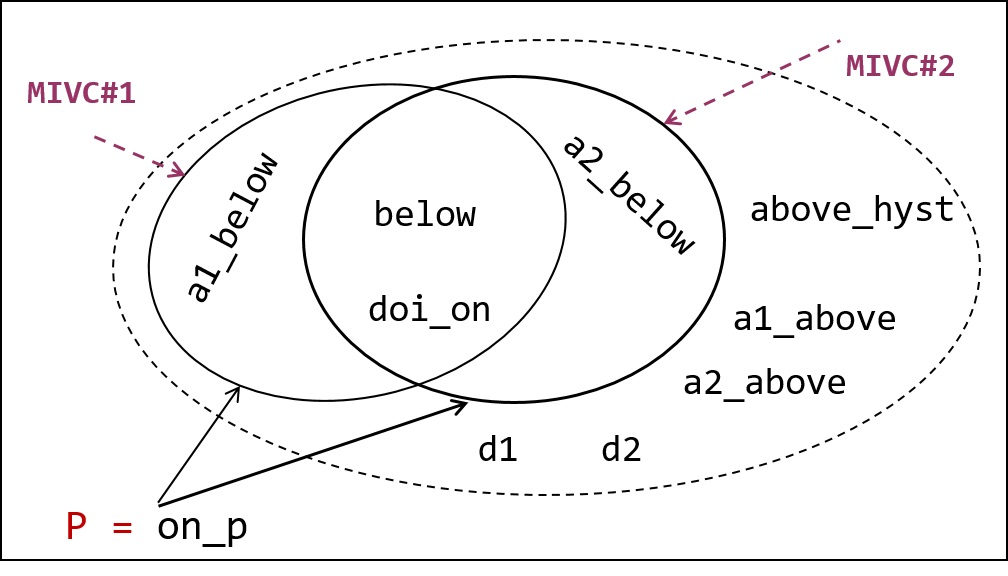
\includegraphics[width=0.9\columnwidth]{figs/ivcs.jpg}
  \vspace{-0.1in}
  \caption{Graphical representation of \mivc s for the model in Fig.~\ref{fig:asw}
  with  $P = ({\small \texttt{on\_p}})$}
  \label{fig:ivcs}
  %\vspace{-0.2in}
\end{figure}

%Distinct IVCs may have common elements, and the intersection of all \mivc s is called the \emph{must} set for $P$.

Generally, an IVC computation technique aims to determine, for any subset $S \subseteq T$, whether $P$ is provable by $S$. Then, a minimal subset that satisfies $P$ is seen as a minimal proof explanation called a minimal Inductive Validity Core.


\subsection{Algorithms for computing one inductive validity core}
%\label{subsec:ivcalg}


\begin{algorithm}[t]
  \SetKwInOut{Input}{input}
  \SetKwInOut{Output}{output}
  \Input{$(I, T)\vdash P$}
  \Output{\mivc for $(I, T)\vdash P$}
  \BlankLine
  $S \leftarrow T$ \\
  \For{$x \in S$} {
    \If{$(I, S\setminus\{x\}) \vdash P$}{
      $S \leftarrow S\setminus \{x\}$
    }
  }
  \Return{S}
\caption{\bfalg: Brute-force algorithm for computing a minimal IVC}
\label{alg:naive}
\end{algorithm}

Lemma \ref{lem:ivc-monotonic} gives us a simple, brute-force algorithm for computing
a minimal inductive validity core, Algorithm \ref{alg:naive} ~(\bfalg). The
resulting set of this algorithm is obviously an inductive validity
core for $(I, T)\vdash P$. The following lemma shows that it is also
minimal.

\begin{lemma}
  The result of Algorithm~\ref{alg:naive} is a minimal inductive validity core
  for $(I, T)\vdash P$.
\end{lemma}
\begin{proof}
  Let the result be $S'$. Suppose towards contradiction that $S'$ is not
  minimal. Then there is an inductive validity core $M$ with $M
  \subset S'$. Take $x \in S'\setminus M$. Since $x \in S'$ it must be
  that during the algorithm $(I, S\setminus\{x\})\vdash P$ is not true
  for some set $S$ where $S' \subseteq S$. We have $M \subset S'
  \subseteq S$ and $x\not\in M$, thus $M \subseteq S\setminus \{x\}$.
  Since $M$ is an inductive validity core,
  Lemma~\ref{lem:ivc-monotonic} says that $S\setminus \{x\}$ is an
  inductive validity core, and so $(I, S\setminus\{x\})\vdash P$. This
  is a contradiction, thus $S'$ must be minimal.
\end{proof}

This algorithm has two problems. First, checking if a safety property
holds is undecidable in general, thus, the algorithm may never terminate
even when the safety property is easily provable over the original
transition system. Second, this algorithm is very inefficient since it
attempts to re-prove the property multiple times.

\begin{algorithm}[t]
  \SetKwInOut{Input}{input}
  \SetKwInOut{Output}{output}
  \Input{$P$ with invariants $Q$ is $k$-inductive for $(I, T)$}
  \Output{\ivc for $(I, T)\vdash P$}
  \BlankLine
  $k \leftarrow \mink(T, P \land Q)$ \\
  $R \leftarrow \reduceinv_k(T, Q, P)$ \\
  \Return{$\minivc_k(I, T, R)$}\\
\caption{\ucalg: Efficient algorithm for computing a nearly minimal inductive validity core from UNSAT cores}
\label{alg:ivc}
\end{algorithm}

The key to a more efficient algorithm is to make better use of the
information that comes out of model checking. In addition to knowing
that $P$ holds on a system $(I, T)$, suppose we also know something
stronger: $P$ with the invariant set $Q$ is $k$-inductive for $(I,
T)$. This gives us the broad structure of a proof for $P$ which allows
us to reconstruct the proof over a modified transition system.
However, we must be careful since this proof structure may be more
than is actually needed to establish $P$. In particular, $Q$ may
contain unneeded invariants which could cause the inductive validity
core for $P \land Q$ to be larger than the inductive validity core for
$P$. Thus before computing the inductive validity core we first try to
reduce the set of invariants to be as small as possible. This
operation is expensive when $k$ is large so as a first step we
minimize $k$. This is the motivation behind
Algorithm \ucalg~(\ref{alg:ivc}).

\begin{figure}
\begin{align*}
  &\bq_1(I, T, P) \equiv \forall s_0.~ I(s_0) \Rightarrow P(s_0) \\
%%%
  &\bq_{k+1}(I, T, P) \equiv \bq_k(I, T, P) \land~ \\
%
  &\hspace{10pt}\left(\forall s_0, \ldots, s_k.~ I(s_0) \land T(s_0,
  s_1) \land \cdots \land T(s_{k-1}, s_k) \Rightarrow P(s_k)\right)
  \\[5pt]
%%%
  &\iq_k(T, Q, P) \equiv (\forall s_0, \ldots, s_k.~\\
%
  &\hspace{10pt} Q(s_0) \land T(s_0,
  s_1) \land \cdots \land Q(s_{k-1}) \land T(s_{k-1}, s_k) \Rightarrow
  P(s_k)) \\[5pt]
%%%
  &\fq_k(I, T, P) \equiv \\
%
  &\hspace{10pt}\bq_k(I, T, P) \land \iq_k(T, P, P)
\end{align*}
\caption{$k$-induction queries}
\label{fig:queries}
\end{figure}

To describe the details of Algorithm~\ref{alg:ivc} we define queries
for the base and inductive steps of $k$-induction
(Fig.~\ref{fig:queries}). Note, in $\iq(T, Q, P)$ we separate the
assumptions made on each step, $Q$, from the property we try to show
on the last step, $P$. We use this separation when reducing the set of
invariants.

We assume that our queries are checked by an SMT solver. That is, we
assume we have a function $\checksat(F)$ which determines if $F$, an
existentially quantified formula, is satisfiable or not. In order to
efficiently manipulate our queries, we assume the ability to create
{\em activation literals} which are simply distinguished Boolean
variables. The call $\checksat(A, F)$ holds the activation literals in
$A$ true while checking $F$. When $F$ is unsatisfiable, we assume we
have a function $\unsatcore()$ which returns a minimal subset of the
activation literals such that the formula is unsatisfiable with those
activation literals held true. In practice, SMT solvers often return a
non-minimal set, but we can minimize the set via repeated calls to
\checksat. We assume both \checksat\ and \unsatcore\ are always
terminating.

\begin{algorithm}[t]
  $k' \leftarrow 1$ \\
  \While{$\checksat(\neg\iq_{k'}(T, P, P)) = \sat$} {
    $k' \leftarrow k' + 1$ \\
    }
  \Return{$k'$} \\
\caption{$\mink(T, P)$}
\label{alg:minimize-k}
\end{algorithm}

The function $\mink(T, P)$ is defined in
Algorithm~\ref{alg:minimize-k}. This function assumes that $P$ is
$k$-inductive for $(I, T)$. It returns the smallest $k'$ such that $P$
is $k'$-inductive for $(I, T)$. We start checking at $k' = 1$ since
smaller values of $k'$ are much quicker to check than larger ones. The
checking must eventually terminate since $P$ is $k$-inductive. We also
only check the inductive query since we know the base query will be
true for all $k' \leq k$. Although we describe each query in
Algorithm~\ref{alg:minimize-k} separately, in practice they can be
done incrementally to improve efficiency.

\begin{algorithm}[t]
  $R \leftarrow \{P\}$ \\
  Create activation literals $A = \{a_1, \ldots, a_n\}$ \\
  $C \leftarrow (a_1 \Rightarrow Q_1) \land \cdots \land (a_n \Rightarrow Q_n)$ \\
  \While{$true$} {
    $\checksat(A, \neg\iq_k(T, C, R))$ \\
    \If{$\unsatcore() = \emptyset$}{
      \Return{R}
    }
    \For{$a_i \in \unsatcore()$}{
      $R \leftarrow R \cup \{Q_i\}$ \\
      $C \leftarrow C \setminus \{a_i \Rightarrow Q_i\}$ \\
    }
  }
\caption{$\reduceinv_k(T, \{Q_1, \ldots, Q_n\}, P)$}
\label{alg:reduce-invariants}
\end{algorithm}

The function $\reduceinv_k(T, \{Q_1, \ldots, Q_n\}, P)$ is defined in
Algorithm~\ref{alg:reduce-invariants}. This function assumes that $P
\land Q_1 \land \cdots \land Q_n$ is $k$-inductive for $(I, T)$. It
returns a set $R \subseteq \{P, Q_1, \ldots, Q_n\}$ such that $R$ is
$k$-inductive for $(I, T)$ and $P \in R$. Like \mink, this function
only checks the inductive query since each element of $R$ is an
invariant and therefore will always pass the base query. A significant
complication for reducing invariants is that some invariants may
mutually need each other, even though none of them are needed to prove
$P$. Thus in Algorithm~\ref{alg:reduce-invariants} we find a minimal
set of invariants needed to prove $P$, then we find a minimal set of
invariants to prove those invariants, and so on. We terminate when no
more invariants are needed to prove the properties in $R$.
Algorithm~\ref{alg:reduce-invariants} is guaranteed to terminate since
$R$ gets larger in every iteration of the outer loop and it is bounded
above by $\{P, Q_1, \ldots, Q_n\}$. As with
Algorithm~\ref{alg:minimize-k}, we describe each query in
Algorithm~\ref{alg:reduce-invariants} separately, though in practice
large parts of the queries can be re-used to improve efficiency.

This iterative lemma determination does not guarantee a minimal
result. For example, we may find $P$ requires just $Q_1$, that $Q_1$
requires just $Q_2$, and that $Q_2$ does not require any other
invariants. This gives the result $\{P, Q_1, Q_2\}$, but it may be
that $Q_2$ alone is enough to prove $P$ thus the original result is
not minimal. Also note, we do not care about the result of \checksat,
only the \unsatcore that comes out of it. Since $P \land Q_1 \land
\cdots \land Q_n$ is $k$-inductive, we know the \checksat call will
always return \unsat.

\begin{algorithm}[t]
  Create activation literals $A = \{a_1, \ldots, a_n\}$ \\
  $T \leftarrow (a_1 \Rightarrow T_1) \land \cdots \land (a_n \Rightarrow T_n)$ \\
  $\checksat(A, \neg\fq_k(I, T, P))$ \\
  $R \leftarrow \emptyset$ \\
  \For{$a_i \in \unsatcore()$}{
    $R \leftarrow R \cup \{T_i\}$
  }
  \Return{R}
\caption{$\minivc_k(I, \{T_1, \ldots, T_n\}, P)$}
\label{alg:minimize-ivc}
\end{algorithm}

The function $\minivc_k(I, \{T_1, \ldots, T_n\}, P)$ is defined in
Algorithm~\ref{alg:minimize-ivc}. This function assumes that $P$ is
$k$-inductive for $(I, T)$. It returns a minimal inductive validity
core $R \subseteq \{T_1, \ldots, T_n\}$ such that $P$ is $k$-inductive
for $(I, R)$. It is trivially terminating. Since
Algorithms~\ref{alg:minimize-k}, \ref{alg:reduce-invariants}, and
\ref{alg:minimize-ivc} are terminating, Algorithm~\ref{alg:ivc} is
always terminating.

Our full inductive validity core algorithm in Algorithm~\ref{alg:ivc}
does not guarantee a minimal inductive validity core. One reason is
that \reduceinv does not guarantee a minimal set of invariants. A
larger reason is that we only consider the invariants that the
algorithm is given at the outset. It is possible that there are other
invariants which could lead to a smaller inductive validity core, but
we do not search for them. The
following theorem shows that minimality checking is at least as hard
as model checking and therefore undecidable in many settings.

\begin{theorem}
\label{thm:minimal-hard}
Determining if an IVC is minimal is as hard as model checking.
\end{theorem}
\begin{proof}
Consider an arbitrary model checking problem $(I, T)\vdash^? P$ where
$P$ is not a tautology. We will construct an IVC for a related model
checking problem which will be minimal if and only if $(I, T)\nvdash
P$. Let $x$ and $y$ be fresh variables. Construct a transition system
with initial predicate $I\land \neg x$ and transition predicate $(x'
\Rightarrow y') \land ((y' \Rightarrow P') \land T)$. The constructed
system clearly satisfies the property $x \Rightarrow P$. Thus $S = \{x'
\Rightarrow y', (y' \Rightarrow P') \land T\}$ is an IVC. $S$ is
minimal if and only if neither $\{x' \Rightarrow y'\}$ nor $\{(y'
\Rightarrow P') \land T\}$ is an IVC. Since $x$ and $y$ are fresh and
$P$ is not a tautology, $\{x' \Rightarrow y'\}$ is not an IVC. Since
$x$ and $y$ are fresh, $\{(y' \Rightarrow P') \land T\}$ is an IVC for
the property $x \Rightarrow P$ if and only if $(I, T)\vdash P$.
Therefore, $S$ is minimal if and only if $(I, T)\nvdash P$.
\end{proof}

When minimality is a matter of concern, we can combine \bfalg\ and \ucalg\ into
a single algorithm which aims to more efficiently determine minimality.  The
hybrid algorithm, \ucbfalg\ (Algorithm \ref{alg:ucbf}), consists of running \ucalg\ to generate an
initial nearly minimal IVC which is then run through \bfalg\ to
attempt to achieve minimality.   For sequential model checking problems with infinite theories, neither \bfalg\ or \ucbfalg\ is guaranteed to terminate, so our implementations simply time out after a set threshold (discussed in more detail in the implementation Section~\ref{sec:impl}).  If no proof can be found within a certain time threshold after removing a model element, we declare that element necessary to the proof. In Section~\ref{sec:experiment} we show that in practice our algorithm is nearly
minimal and much more efficient than the brute-force approach.

\begin{algorithm}
  \SetKwInOut{Input}{input}
  \SetKwInOut{Output}{output}
  \Input{$(I, T) \vdash P$}
  \Output{Minimal IVC for $(I, T) \vdash P$}
  \BlankLine
  $S \leftarrow \ucalg((I, T) \vdash P)$ \\
  \For{$x \in S$} {
    \If{$(I, S\setminus\{x\}) \vdash P$}{
      $S \leftarrow S\setminus \{x\}$
    }
  }
  \Return{S}
\caption{An abstract representation of \ucbfalg }
\label{alg:ucbf}
\end{algorithm}


%%% Local Variables:
%%% mode: latex
%%% TeX-master: "main.tex"
%%% End

%%  LocalWords:  Lustre \emph{iff} TODO invariants Minimality BaseQuery IVC
%%  LocalWords:  InductiveQuery FullQuery MinimizeK ReduceInvariants
%%  LocalWords:  MinimizeIVC CheckSat UnsatCore UNSAT UC UCBF
%%  LocalWords:  IndQuery MinimizeIvc minimality




\subsection{Algorithm for computing all minimal inductive validity cores}
\label{sec:allivcs}
\newcommand{\unknown}{\textsc{Unknown}}
\newcommand{\adequate}{\textsc{Adequate}}
\newcommand{\inadequate}{\textsc{Inadequate}}

\newcommand{\true}{\textsc{True}}
\newcommand{\false}{\textsc{False}}

Now, we turn to the problem of finding {\em all} minimal IVCs.  By definition, this approach allows us to find the {\em minimum} IVC in terms of number of elements (which may not be unique), and it allows us to explore the {\em diversity} of proofs for a particular property.

Considering the definition of a \mivc, a brute-force technique for enumerating all \mivc s would be the same as exploring the power set of $T$ (denoted by $ \mathcal{P}(T) $).
Basically, the algorithm needs to explore the provability of a
given property by any subset of $T$, which would be computationally expensive.  Our approach is an adaptation of the the work of MARCO for generating all minimal unsatisfiable subsets (MUSes) in~\cite{marco2016fast}, and only needs to explore a (small) portion of $\mathcal{P}(T)$ in order to compute $AIVC$.  In fact, it can be viewed as an instantiation of the MARCO proof schema for the richer theory of sequential model checking.  We begin by introducing several additional notions and definitions, most of which are analogous or equivalent to those in~\cite{marco2016fast}.


\begin{definition}{\emph{Maximal Inadequate Set (\mis):}}
  \label{def:mis}
  $S \subset T$ for $(I, T) \vdash P$ is a Maximal Inadequate Set (\mis) iff
  $(I, S) \nvdash P$ and $\forall T_i \in T\setminus S.~ (I, S\cup\{T_i\}) \vdash P$.
\end{definition}

%\begin{definition} {\emph{Adequacy:}}
%\label{def:adeq}
Given $(I, T) \vdash P$, for every $S \in \mathcal{P}(T)$, we have either $(I, S) \vdash P$ or $(I, S) \nvdash P$. In the former case, we say $S$ is \textbf{adequate} for $P$; in the latter, we say that $S$ is \textbf{inadequate} for the proof of $P$.
%\end{definition}
Note that every \ivc ~is an adequate set for $P$, and every \mis ~is an inadequate set.

%\begin{definition}{\emph{Minimal Correction Set (MCS):}}
%  \label{def:mcs}
%  $S \subset T$ for $(I, T) \vdash P$ is a Minimal Correction Set (MCS) iff
%  $(I, T \setminus S) \nvdash P$ and $\forall T_i \in S.~ (I, (T \setminus S)\cup \{T_i\}) \vdash P$.
%\end{definition}

%It should be mentioned that minimality and maximality are about minimum or maximum cardinality subsets.
%Note that $MCS$ is more of syntactic sugar that specifies sets that can also be specified by $MIS$; i.e. for any $MIS$ of $T$, there is a corresponding $MCS$ such that adding any element of that $MCS$ to the $MIS$, makes the property provable by the $MIS$.
%And, that's why it is called the ``minimal correction'' set.

\begin{lemma}
\label{lem:adeq}
For $(I, T) \vdash P$, if $S \subseteq T$ is adequate for property $P$, then all of its supersets are adequate for $P$ as well:
\allowbreak $$\forall S_1 \subseteq S_2 \subseteq T.~ (I, S_1) \vdash P \Rightarrow (I, S_2) \vdash P$$
\end{lemma}
\begin{IEEEproof}
From $S_1 \subseteq S_2$ we have $S_2 \Rightarrow S_1$. Thus the
  reachable states of $(I, S_2)$ are a subset of the reachable states
  of $(I, S_1)$.
\end{IEEEproof}

\begin{corollary}
\label{lem:inadeq}
For $(I, T) \vdash P$, if a given subset $S$ is inadequate, then all of its subsets are inadequate as well:
\allowbreak $$\forall S_1 \subseteq S_2 \subseteq T.~ (I, S_2) \nvdash P \Rightarrow (I, S_1) \nvdash P$$
\end{corollary}
\begin{IEEEproof}
  Immediate from Lemma \ref{lem:adeq}.
\end{IEEEproof}
%\begin{IEEEproof}
%Given the fact that $(I, T) \vdash P$ and $S_2$ is inadequate,
%there is a correction set $C \subseteq (T\setminus S_2)$ such that
%$C \cup S_2$ is adequate, which implies every $S' \subseteq (T \setminus C)$ is inadequate.
%So, since $S_1 \subset S_2 \subseteq (T \setminus C)$, set $S_1$ is also inadequate.
%\end{IEEEproof}

%\begin{corollary}
%$\forall S \in AIVC(P)$, S is a minimal adequate set for $P$.
%\end{corollary}
%\begin{IEEEproof}
%  Immediate from the definitions of $IVC$ and $AIVC$, and Lemma \ref{lem:adeq}.
%\end{IEEEproof}

The basic idea behind an algorithm for computing $AIVC(P)$ is the same
as exploration of $\mathcal{P}(T)$, with two major performance
improvements. First, Lemma~\ref{lem:adeq} and
Corollary~\ref{lem:inadeq} are used to block large portions of
$\mathcal{P}(T)$ from consideration. For example, if a set $S \in
\mathcal{P}(T)$ is found to be inadequate, then all subsets of $S$ are
also inadequate and do not need to be explicitly considered. Second,
if a set $S \in \mathcal{P}(T)$ is found to be adequate, then a fast
algorithm (such as \ucalg\ from \cite{Ghass16}) is used to find a
smaller $S' \subseteq S$ which is still adequate. This feeds into the
first optimization since now all supersets of $S'$ rather than $S$ are
blocked from future consideration.

To guide our algorithm, we now introduce a way of exploring
$\mathcal{P}(T)$ which allows us to eliminate all subsets or supersets
of any given set. We use a Boolean expression called $map$, which is
in conjunctive normal form (CNF) and built gradually as the algorithm
proceeds. Satisfying assignments for $map$ correspond to elements of
$\mathcal{P}(T)$. For each $S \in \mathcal{P}(T)$ that the algorithm
determines to be adequate or inadequate, a corresponding clause is
added to $map$ which blocks $S$ and all supersets or subsets,
respectively, from consideration. When a clause is added to $map$, the
corresponding $S \in \mathcal{P}(T)$ is called \emph{explored}.
The supersets or subsets of $S$ which are blocked from
consideration are called \emph{excluded}. The remaining elements
of $\mathcal{P}(T)$ are \emph{unexplored}.

More precisely, given $T$ with $n$ top-level conjuncts, we define an
ordered set of activation literals $\mathcal{A} = \{a_1, \ldots,
a_n\}$, where each $a_i$ has type Boolean. We assume the function
$\actlit : T \rightarrow \mathcal{A}$ is a bijection assigning every
$T_i \in T$ to an $a_i \in \mathcal{A}$ and vice versa. Then, a $map$
for $AIVC(P)$ is a CNF formula built over the elements of
$\mathcal{A}$ such that:
\begin{itemize}
  \item Initially $map$ is $\top$ since all of $\mathcal{P}(T)$ is unexplored.

  \item When $map$ is satisfiable, a model of it is a set
  $M \in \mathcal{P}(\mathcal{A})$ consisting of those $a \in
    \mathcal{A}$ which are assigned $true$.

  \item Every model $M$ of $map$ corresponds to a set $S \in \mathcal{P}(T)$ such that
$S = \bigcup_{a_i \in M} \actlit ^{-1} (a_i)$ and $M = \bigcup_{T_i \in S} \actlit(T_i)$.
\vspace{0.05in}
  \item For every explored set $S \in \mathcal{P}(T)$:
  \begin{itemize}
    \item if $S$ is adequate for $P$, then $map$ contains a clause
      $\bigvee_{T_{i}\in S} \neg {\actlit (T_i)}$. This clause blocks
      all supersets of $S$ from future consideration which is
      consistent with Lemma~\ref{lem:adeq}.

    \item if $S$ is inadequate for $P$, then $map$ contains a clause
      $\bigvee_{T_{i}\in (T \setminus S)} \actlit (T_i)$. This clause
      blocks all subsets of $S$ from future consideration which is
      consistent with Corollary~\ref{lem:inadeq}.
  \end{itemize}
\end{itemize}


\begin{lemma}
\label{lem:map:sound}
When $map$ is satisfiable with model $M$, set $S = \bigcup_{a_i \in M} \actlit ^{-1} (a_i)$ is not equal to any adequate or inadequate explored set, nor a subset (superset) of any
inadequate (adequate) explored set in $\mathcal{P}(T)$.
\end{lemma}
\begin{IEEEproof}
Proof by contradiction. Case 1: Suppose there is an adequate set $Ex \subseteq S$ that has been already explored. Therefore, according to the definition, $map$ contains a clause $C = \bigvee_{T_{i}\in Ex} \neg {\actlit (T_i)}$, and since $Ex \subseteq S$, it is impossible for the model $M = \bigcup_{T_i \in Ex} \actlit (T_i)$ to satisfy $C$; hence, the assumption is false.

Case 2: Suppose there is an inadequate set $Ex$ such that $S \subseteq Ex$ and $Ex$ has been already explored. Therefore, according to the definition, $map$ contains a clause $C = \bigvee_{T_{i}\in (T \setminus S)} \actlit (T_i)$, and since $S \subseteq Ex$, it is impossible for the model $M = \bigcup_{T_i \in S} \actlit (T_i)$ to satisfy $C$; so, the assumption is false.

From Case 1 and Case 2, there is no model of $map$ whose corresponding set in $\mathcal{P}(T)$ is a non-strict subset (superset) of any inadequate (adequate) explored set.
\end{IEEEproof}

%Next, we tie the {\em map} results back to the minimal IVCs problem. Note that from Theorem~\ref{thm:minimal-hard}, finding a minimal IVC may be undecidable if the original checking problem is undecidable.  In most cases, if we are able to prove a property against a full model, we are able to conclusively determine its MIVCs, but it is not guaranteed.  For a given set $S$, if our implementation is unable to prove the property, we conservatively assume that the property is falsifiable and note to the user that the results may be approximate.  We discuss how our implementation manages undecidability in more detail in Section~\ref{sec:impl}.

\begin{lemma}
\label{lem:map:comp}
For $(I, T) \vdash P$, $map$ is satisfiable iff
at least one $S \in AIVC(P)$ or one \mis\ of $T$ is unexplored.
\end{lemma}
\begin{IEEEproof}
Let $map$ is satisfiable with a model $M$, and let $S = \bigcup_{a_i
  \in M} \actlit ^{-1} (a_i)$ be the corresponding set of
$\mathcal{P}(T)$. If $S$ is adequate, then it contains a \mivc. That
\mivc\ must not be explored since otherwise $S$ would have been blocked
from consideration. The \mivc\ must not be excluded since it is not a
strict superset of any adequate set (by minimality) nor a subset of
any inadequate set (by Corollary~\ref{lem:adeq}). Thus the \mivc\ must
be unexplored. The case where $S$ is inadequate is symmetric.

In the other direction, let $S \subseteq T$ be an unexplored \mivc.
Then consider the model $M = \bigcup_{T_i\in S} \actlit(T_i)$. We will
show that each clause of $map$ is satisfied by $M$. There are two
types of clauses to consider. A clause $\bigvee_{T_{i}\in S'} \neg
{\actlit (T_i)}$ is in $map$ only if $S'$ is adequate. $M$ would
falsify this clause only if $S' \subseteq S$ which is impossible by
minimality of $S$. A clause $\bigvee_{T_{i}\in (T \setminus S')}
\actlit (T_i)$ is in $map$ only if $S'$ is inadequate. $M$ would
falsify this clause only if $S \subseteq S'$ which is imposssible by
Corollary~\ref{lem:inadeq}. Thus $M$ is a model for $map$. The case
for an unexplored \mis\ is symmetric.
\end{IEEEproof}


%\begin{lemma}
%\label{lem:map:comp}
%For $(I, T) \vdash P$, $map$ is unsatisfiable \emph{iff} all $S \in AIVC(P)$ and all $MIS$es of $T$ (and thus every $S \in \mathcal{P}(T)$) have been explored.
%\end{lemma}
%\begin{IEEEproof}
%As with any CNF formula, $map$ is unsatisfiable \emph{iff} every complete assignment falsifies at least one of its clauses. Clauses in $map$ have special structure;
%according to definition, every clause contains a set of either entirely negative literals or entirely positive; when a set $S$ corresponding to a model $M$ of map is explored, if $S$ is adequate, it means that it contains necessary elements of $T$ to prove $P$, which
%are added to $map$ as a new clause containing \emph{negative} activation literals of $S$. However, when
%$S$ is inadequate, it means that $S$ lacks a correction set $C$ of $T$ so to prove $P$.
%And, in this case, a new clause containing \emph{positive} activation literals of $C$ is added to $map$. Generally, similar to the elements of adequate sets, elements of correction sets are also essential part of some proof, which means eventually, negative literals added from adequate sets will have their own  positive form added from the correction sets (and vice versa).
%Therefore, every complete assignment falsifies at least one clause in $map$ \emph{iff} every
%member of $\mathcal{P}(T)$ is dominated by some adequate or inadequate set.
%And, considering the definitions of $IVC$ and $MIS$,  every member of $\mathcal{P}(T)$ is dominated by some set \emph{iff} all \ivc s and \mis es have been explored. According to definition of $map$, when all $IVC$s and $MIS$es are covered, every $S \in \mathcal{P}(T)$ will be covered as well.
%\end{IEEEproof}

\begin{corollary}
\label{cor:map:cc}
For $(I, T) \vdash P$, $map$ is unsatisfiable iff every $S \in
\mathcal{P}(T)$ has been explored or excluded.
\end{corollary}
\begin{IEEEproof}
Immediate from the definition of $map$ and Lemma \ref{lem:map:comp}.
\end{IEEEproof}


Algorithm~\ref{alg:aivc} shows the process of capturing all \mivc s,
which are kept in set $A$, along with a warning flag, explained below.
In line 2, we create the set of activation
literals used by function \actlit . Line 3 initializes $map$ with
$\top$ over the set of literals we have. The main loop of state
exploration starts at line 4 and continues until $map$ becomes \unsat
which means all the \mivc s have been found. We assume we have a
function \checksat ~that determines if an existentially quantified
formula is satisfiable or not.
%\footnote{We assume readers are familiar
%  with the Boolean satisfiability problem, which is the problem of
%  determining whether there exists an assignment that satisfies a
%  given propositional formula. For more information, refer to
%  \cite{cook1971complexity}.}
%$$\checksat : Boolean \rightarrow \{ true~(\sat), false~(\unsat) \}$$
As long as $map$ is satisfiable, the algorithm computes a
\emph{maximal} \sat model for it (line 5). In this context,  a maximal SAT model is a
model with as many $true$ assignment as possible without violating a
clause; this problem, is equivalent
to the MaxSAT problem, which has been well studied in the
literature \cite{davies2011solving,
  morgado2013iterative}.\footnote{MaxSAT is defined as the problem of satisfying as many
(weighted) clauses as possible in a SAT instance. For $N$
variables, similar to the MaxSAT problem, each clauses is weighted at $N+1$ and extra unit-weight clauses are added forcing each variable to $1$.} So, we assume there is a method by which we
are able to have a maximal model of $map$. Line 6 extracts a set $M
\in \mathcal{P} (\mathcal{A})$ of literals assigned to $true$ in the
model. Then, we need to obtain the corresponding set of $S$ in
$\mathcal{P}(T)$, which is done with function $\actlit ^{-1}$ in line
7.

We also assume there is a function \isadeq\ that checks whether or
not $P$ is provable by a given subset of $T$.  Note that from Theorem~\ref{thm:minimal-hard}, finding a minimal is undecidable if the original checking problem is undecidable.  Thus, for undecidable model checking problems, \isadeq\  can return \unknown ~(after a user-defined timeout) as well as \adequate\ or \inadequate.
For a given set $S$, if our implementation is unable to prove the property, we conservatively assume that the property is falsifiable and set a warning flag $w$ to the user that the results may be approximate.  %Using this function, the
%adequacy of $S$ is determined in line 8.
if $S$ is adequate, a \mivc
~is computed by \getivc ~and added to set $A$ (lines 10-11).\footnote{Note
  that \isadeq ~can be any method that verifies a safety property,
  such as K-induction, and the \getivc\ function can be any function
  that returns an (approximately) minimal IVC, such as the \ucalg\ or
  \ucbfalg\ algorithms. The only requirement is
  that it follows the definition of an inductive validity core, that
  is: $S' \leftarrow \getivc (P, S)$ implies that $S' \subseteq S$ and
  $(I, S') \vdash P$.} In this case $map$ is constrained by a new
clause in a way described before and shown in line 12. However, in the
case that $S$ is inadequate or unknown, $map$ is constrained by the corresponding
literals from $T \setminus S$ in line 14.  Finally, if $S$ is unknown, the warning flag $w$ is set to true, as the results may be approximate (lines 15-16).

\begin{algorithm}[t]
  \SetKwInOut{Input}{input}
  \SetKwInOut{Output}{output}
  \Input{$(I, T) \vdash P$}
  \Output{$AIVC (P)$, Approximation warning flag $w$}
  \BlankLine
  $A \leftarrow \varnothing$; $w \leftarrow \false$ \\
  Create activation literals $\{a_1, \ldots, a_n\}$ \\
 % $map \leftarrow true$ \\
  $map \leftarrow \top$ \\
 % $L \leftarrow \varnothing$ \\
  \BlankLine

  \While{$\checksat (map) = \sat$} { \label{alg:aivc:checksat}
    $model \leftarrow $ build a maximal model of $map$  \label{alg:aivc:maxsat} \\
    $M \leftarrow$ extract the set of variables assigned $true$ in $model$ \label{alg:aivc:assignm}\\
    $S \leftarrow \bigcup_{a_i \in M} \actlit ^{-1}(a_i)$ \label{alg:aivc:assigns}\\
    $res \leftarrow \isadeq (P, S)$ \\
%\BlankLine
    \If{$res = \adequate$}{
    %\BlankLine
      $S' \leftarrow \getivc (P, S)$ \label{alg:aivc:getivc} \\
      $A \leftarrow A \cup \{S'\}$ \label{alg:aivc:addset}\\
      $map \leftarrow map \wedge (\bigvee_{T_{i}\in S'} \neg {\actlit (T_i)})$ \label{alg:aivc:aadd}
    }
    \Else{
      $map \leftarrow map \wedge (\bigvee_{T_{i}\in (T \setminus S)} \actlit (T_i))$ \label{alg:aivc:iadd} \\
      \If{$res = \unknown$} {
        $w \leftarrow \true$
      }
    %  $L \leftarrow L \cup (\bigcup_{T_i \in C} T_i)$
    }
  }
  \Return{$A, w$}
\caption{Algorithm \aivcalg ~for computing $AIVC$}
\label{alg:aivc}
\end{algorithm}


\begin{theorem}
\label{theorem:termination}
  Algorithm~\ref{alg:aivc} will terminate.
\end{theorem}
\begin{IEEEproof}
We assume that \isadeq\ has a finite timeout, so all operations within the
loop require finite time.  Each iteration of the while loop in Algorithm~\ref{alg:aivc} blocks at least one element of $\mathcal{P}(T)$ which was not previously
blocked. Since $\mathcal{P}(T)$ is finite, the algorithm terminates.
\end{IEEEproof}

\begin{theorem}
\label{theorem:aivc}
  If no approximation warning is returned ($w$ is $\false$), Algorithm \ref{alg:aivc} enumerates all \mis es and \mivc s.
\end{theorem}

\begin{IEEEproof}
By Theorem~\ref{theorem:termination} the algorithm terminates. This
means $map$ is eventually unsatisfiable.  If $w = \false$ then all model checking problems are solved definitively (no \unknown\ results), so by Lemma~\ref{lem:map:comp},
all \mis es and \mivc s are either explored or excluded.
However, by maximality and Lemma~\ref{lem:adeq}, an \mis~ can never be
excluded. Similarily, by minimality and Corollary~\ref{lem:inadeq}, a
\mivc~ can never be excluded. Thus all \mis es and \mivc s are
explored and are elements of $A$ by the end of the algorithm.



%% We first note that for any model, the number of possible \mis es and adequate sets is finite, so we can do induction on the number of remaining sets to be added to $map$.
%% Suppose that $x$ is an undiscovered \mivc\ in $map$ after some number of iterations (including 0) of the algorithm.

%% Base case: Suppose that $\checksat$ is unsatisfiable.  By Lemma~\ref{lem:map:comp}, this contradicts our assumption that $x$ is an undiscovered \ivc\ in $map$.

%% Inductive case: $map$ is satisfiable, so the loop proceeds.  In each iteration of the \texttt{while} loop, Algorithm \ref{alg:aivc} extracts a model $M$ from $map$ in line~\ref{alg:aivc:maxsat}, which has not been previously explored, by Lemma~\ref{lem:map:sound}.  If $M$ is inadequate, then it yields a \mis\ (by virtue of using MaxSAT).  This \mis\ is blocked in line~\ref{alg:aivc:iadd}.  By Lemma~\ref{lem:map:comp}, $map$ is still satisfiable, the loop proceeds with a smaller number of remaining sets to add to $map$, and by induction, $x$ is eventually discovered.  Suppose alternately that $M$ is adequate.  If $M = x$, we are finished.  Alternately, $M \neq x$, so $M$ is blocked in line~\ref{alg:aivc:aadd}, $map$ is still satisfiable, and by induction $x$ is eventually discovered.

%% The case where $x$ is an undiscovered \mis\ in $map$ is essentially the same.



%As there are a finite number of model constraints, there are a finite number of \mis es and \ivc s.
%
%If the model is inadequate, then it yields a \mis (by virtue of using MaxSAT).  If the model is adequate, then the model
%yields either a minimal inductive validity core, or a superset of a minimal inductive validity core.  In either adequacy case, the clause is blocked for future exploration (lines~\ref{alg:aivc:aadd} and~\ref{alg:aivc:iadd}).  If any remaining minimal \ivc s or \mis es remain, then , $map$ is still satisfiable, and the loop continues iterating (line~\ref{alg:aivc:checksat}).


%By Lemma~\ref{lem:map:comp},
%
%it yields an
%inductive validity core, which may be a subset of an
%
%which is added back into the map in line~\ref{alg:aivc:iadd},
%so subsequent iterations must
%
%explores a set which is either a \mis\ (by virtue of using MaxSAT) or is an adequate set.
%These sets have not explored before according to Lemma \ref{lem:map:sound}.  If the set is inadequ
%So, in each iteration a new adequate or maximal inadequate member of $\mathcal {P}(T)$ is explored.  Therefore, the loop continues as long as there is any \ivc\ or
%\mis\ not yet found.
\end{IEEEproof}

Note that none of the proofs above require that \getivc\ returns a minimal IVC.
As shown in Section \ref{sec:experiment}, it is computationally cheap to find an
approximately minimal \ivc\ using the algorithm \ucalg; however, using the better,
usually minimal \ivc\ using the \ucbfalg\ algorithm is computationally expensive.  For efficiency
reasons, it is much better to use the approximate \ucalg\ algorithm to compute the set of
all \mivc s.  The \ucbfalg\ algorithm attempts to repeatedly prove the property by brute-force removing elements (BF = ``brute force''), so does much of the work of Algorithm~\ref{alg:aivc} in a way that is not effective towards finding other IVCs.  The overhead of the \ucalg\ algorithm is on average 31\% over the baseline proof, as opposed to 2276\% for the \ucbfalg\ algorithm.  In addition, the average increase in size of IVCs returned by \ucalg\ is approximately 8\% of the \ucbfalg\ algorithm.

On the other hand, if \getivc ~does not return minimal adequate sets, at the end of the process,
set $A$ may contain both \mivc s and some supersets of \mivc s. To make sure that the algorithm only returns
the minimal adequate sets (\mivc s), all we need is to remove any supersets of other sets in $A$.  We can do this ``on the fly'' by changing
line~\ref{alg:aivc:addset} to the following:
$A \leftarrow A \cup \{S'\} \setminus \{ S~|~S \in A \wedge S' \subset S \}$.
Obviously, the closer to minimal the results of \getivc ~are,
the fewer iterations are required for Algorithm 1 to terminate.  Each non-minimal adequate set returned by \textsc{GetIVC} will induce an additional iteration for Algorithm 1.



%\subsection{Minimality of Inductive Validity Cores}
\label{subsec:minimality}
\newcommand{\ucalg}{\texttt{\small{IVC\_UC}}}
\newcommand{\ucbfalg}{\texttt{\small{IVC\_UCBF}}}

To compute all $IVC$s of a given property, the \aivcalg ~algorithm
 makes a major assumption on the outcome of the \getivc ~module;
it assumes \getivc ~returns \emph{minimal} Inductive Validity Cores.
However, as shown in \cite{Ghass16},
determining  the minimality of  an  $IVC$ is  hard. Although the $IVC$ generation algorithm proposed by Ghassabani et al. \cite{Ghass16}, called \ucalg ,
is efficient and fast, it does not guarantee minimality;
i.e. an $IVC$ obtained from \ucalg ~is either minimal or approximately minimal.
In the \ucalg ~algorithm, $IVC$s are built upon inductive proofs,
which usually rely on additional
lemmas (or invariants) derived by the model checking algorithms
for strengthening the property and proving it
inductively.
Depending on the structure of the inductive
proofs, an $IVC$ computed by \ucalg ~might still not be minimal.
They also proposed another algorithm that guarantees
the minimality of an $IVC$ \cite{Ghass16}, called \ucbfalg, which is a lot more expensive than the \ucalg. The \ucbfalg ~takes an $IVC$ generated by
the \ucalg ~as input and then, minimizes it brute-forcefully. In this section,
first we show that the \aivcalg ~algorithm is correct even if
 the \getivc ~module does not guarantee minimality.
Then, we mention how to modify Algorithm \ref{alg:aivc}
 such that the output set $A$ only contains the \textbf{minimal} $IVC$s.

%\begin{algorithm}
%  \SetKwInOut{Input}{input}
%  \SetKwInOut{Output}{output}
%  \Input{$(I, T) \vdash P$}
%  \Output{Minimal IVC for $(I, T) \vdash P$}
%  \BlankLine
%  $S \leftarrow \ucalg((I, T) \vdash P)$ \\
%  \For{$x \in S$} {
%    \If{$(I, S\setminus\{x\}) \vdash P$}{
%      $S \leftarrow S\setminus \{x\}$
%    }
%  }
%  \Return{S}
%\caption{An abstract representation of \ucbfalg \cite{Ghass16}}
%\label{alg:ucbf}
%\end{algorithm}

\begin{theorem}
\label{theorem:ivc-not-min}
  Algorithm \ref{alg:aivc} enumerates all minimal Inductive Validity Cores
  even if \getivc ~does not guarantee minimality of an Inductive Validity Core.
\end{theorem}
\begin{proof}
In an iteration of the \texttt{while} loop that $\isadeq (P, M)$ is $true$,
let \getivc ~returns a set $S'$ which is not minimal:
$\exists \mathcal{M} \subset S'.~ (I, \mathcal{M}) \vdash P$ and
$\forall T_i \in \mathcal{M} . ~ (I, \mathcal{M} \setminus \{T_i\}) \nvdash P$.
Therefore, there is an unexplored set $S \supseteq \mathcal{M}$ that all its supersets have already been explored, which means
$map$ is still satisfiable.
So, eventually there will be a model of $map$ that makes $M = S$ in line 7.
Again at that point, suppose \getivc ~returns an adequate set $S''$ which is not minimal.
We know that
  $\mathcal{M} \subset S'' \subseteq S \wedge S'' \neq S' \wedge |S''| \leq |S'|$.
  Previously, set $S'$ marked all its supersets as explored. And now, the
  same thing happens with $S''$.
  In the worst case scenario, \getivc
   ~explores all the supersets of $\mathcal{M}$
   before generating $\mathcal{M}$; hence with the same reasoning,
  eventually, all the supersets of $\mathcal{M}$ will be explored, and there will be a model of $map$ that makes $M = \mathcal{M}$ in line 7,
  which results in a minimal $IVC$ by \getivc ~(because $\mathcal{M}$ is minimal itself).
  Now,  $\mathcal{M}$  prunes itself from the $map$.
  This reasoning can be applied to all minimal Inductive Validity Cores.
  Therefore, Algorithm \ref{alg:aivc} explores all minimal adequate sets even if \getivc ~
  does not guarantee minimality.
\end{proof}

\begin{theorem}
 Algorithm \ref{alg:aivc} will terminate even if \getivc ~does not guarantee minimality.
\end{theorem}
\begin{proof}
  Immediate from Theorem \ref{theorem:ivc-not-min}, \ref{theorem:aivc}, and \ref{theorem:termination}.
\end{proof}

Although we have proved that \getivc ~does not have to return minimal sets,
with the current version of the \aivcalg ~algorithm, if \getivc ~does not
return minimal adequate sets, at the end of the process,
 set $A$ may contain some supersets of
minimal IVCs as well. So, to make sure that the algorithm only returns
the minimal adequate sets ($IVC$s), all we need is to
remove supersets before returning $A$; for example, adding the following code snippet after line 9 of Algorithm \ref{alg:aivc} serves this purpose:

\vspace{0.09in}
\indent  \For{$X \in A$}{
\indent        \If{$S' \subset X$}{ $A \leftarrow A \setminus \{X\}$}
\indent      }
\vspace{0.09in}
\noindent Obviously, the closer to minimal the results of \getivc ~are,
the more quickly the search space shrinks and Algorithm \ref{alg:aivc} terminates.

%
%\begin{algorithm}[t]
%  \SetKwInOut{Input}{input}
%  \SetKwInOut{Output}{output}
%  \Input{$(I, T) \vdash P$}
%  \Output{$AIVC (P)$}
%  \BlankLine
%  $A \leftarrow \varnothing$\\
%  Create activation literals $\{a_1, \ldots, a_n\}$ \\
% % $map \leftarrow true$ \\
%  $map \leftarrow \top$ \\
% % $L \leftarrow \varnothing$ \\
%  \BlankLine
%
%  \While{$\checksat (map)$} {
%    $model \leftarrow $ build a maximal model of $map$ \\
%    $M \leftarrow$ extract the set of variables assigned $true$ in $model$ \\
%    $M \leftarrow \bigcup_{a_i \in M} \actlit ^{-1}(a_i)$ \\
%\BlankLine
%    \If{$\isadeq (P, M)$}{
%    \BlankLine
%      $S' \leftarrow \getivc (P, M)$ \\
%
%      \For{$X \in A$}{
%        \If{$S' \subset X$}{ $A \leftarrow A \setminus X$}
%      }
%      $A \leftarrow A \cup S'$ \\
%
%      $map \leftarrow map \wedge (\bigvee_{T_{i}\in S'} \neg {\actlit (T_i)})$
%    }
%    \Else{
%      $map \leftarrow map \wedge (\bigvee_{T_{i}\in (T \setminus M)} \actlit (T_i))$ \\
%    %  $L \leftarrow L \cup (\bigcup_{T_i \in C} T_i)$
%    }
%  }
%  \Return{$A$}
%\caption{Modified version of the \aivcalg ~algorithm that
%guarantees $AIVC(P)$ contains minimal Inductive Validity Cores}
%\label{alg:aivc2}
%\end{algorithm} 
%\begin{algorithm}[t]
%  $k' \leftarrow 1$ \\
%  \While{$\checksat(\neg\iq_{k'}(T, P, P)) = \sat$} {
%    $k' \leftarrow k' + 1$ \\
%    }
%  \Return{$k'$} \\
%\caption{$\mink(T, P)$}
%\label{alg:minimize-k}
%\end{algorithm}


%\begin{theorem}
%\label{thm:minimal-hard}
%\end{theorem}
%\begin{IEEEproof}
%\end{IEEEproof}

%%% Local Variables:
%%% mode: latex
%%% TeX-master: "main.tex"
%%% End:


